\documentclass{article}
\usepackage{graphicx} % Required for inserting images
\usepackage{float} %required for the positioning [H]


\title{Relazione Progetto Tecnologie Internet}
\author{ }
\date{Maggio 2024}

\begin{document}

\maketitle
\tableofcontents

% frontend + flappy + fonti
% backend + snake + dependency

%ordine:
%dependency -> front -> back -> fonti


\section{Dependencies}
In questa sezione si trovano tutti quei pacchetti che vanno installati per il corretto funzionamento dell’applicazione:

\subsection{Tecnologie da installare}
Essendo il progetto svolto in React e Flask dobbiamo andare ad installare rispettivamente node e python:
\begin{itemize}
    \item install node
    \item install python
\end{itemize}

\subsection{Pacchetti da installare lato client}
Ora che abbiamo i linguaggi di programmazione installati dobbiamo spostarci nella cartella “frontend” tramite terminale e andare ad installare i seguenti pacchetti:
\begin{itemize}
    \item npm install
    \item npm i react-router-dom
    \item npm axios
\end{itemize}

\subsection{Pacchetti da installare lato server}
Passando invece alla cartella “backend” andiamo ad installare tramite terminale i seguenti pacchetti:
\begin{itemize}
    \item pip3 install flask
    \item pip3 install Flask-Cors
\end{itemize}





\section{Frontend}



\section{Backend}

\subsection{Import e setup}

\begin{figure}[H]
    \centering
    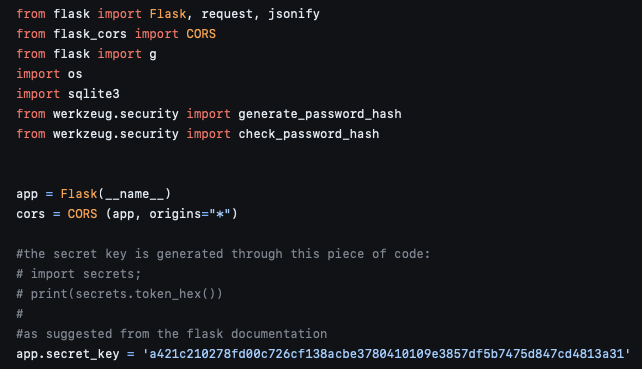
\includegraphics[width=0.9\textwidth]{images/import.png}
\end{figure}

\subsubsection{Import}
Il nostro file inizia con l’import di tutte le librerie che andremo ad usare: lato server, per la crittografia e per il database.

In particolare andiamo ad importare il framework Flask, scelto per la sua semplicità e minimalismo, inoltre andiamo ad importare tutte quelle librerie che ci servono per interagire con il client ricevendo ed inviando rispettivamente con “request" e "jsonify".

La seconda sezione di import riguarda tutto ciò di cui abbiamo bisogno per il database: g è un oggetto che useremo per salvare, temporaneamente, e condividere i dati in parti differenti della nostra applicazione.

L’import del modulo os serve per gestire la posizione dei file, in particolare del database in questo caso.

Come ultimo import in questa sezione abbiamo il modulo sqlite3, che ci consente di creare, inizializzare e utilizzare il nostro database.


Le utile due righe nella sezione di import servono per i moduli necessari rispettivamente alla creazione e al controllo dell’hash associati alla crittografia della password. 

\subsubsection{Setup di base}
Le prime due righe di codice servono ad inizializzare la nostra applicazione in flask e a configurare CORS (Cross-Origin Resource Sharing), quest'ultimo ci serve per consentire richieste da fonti esterne. 
L’asterisco associato al parametro origins specifica che le richieste possano avvenire da qualunque origine (dominio o indirizzo IP).

L’ultima riga di questa sezione è quella che riguarda l’inizializzazione della chiave segreta che useremo per la crittografia della password.

\subsection{Setup Database}
Questa sezione di codice, invece, è dedicata alla creazione, inizializzazione e chiusura del database sqlite3, già presente in Flask e ottimo per gestire carichi di lavoro moderati come in questo caso:
\begin{figure}[H]
    \centering
    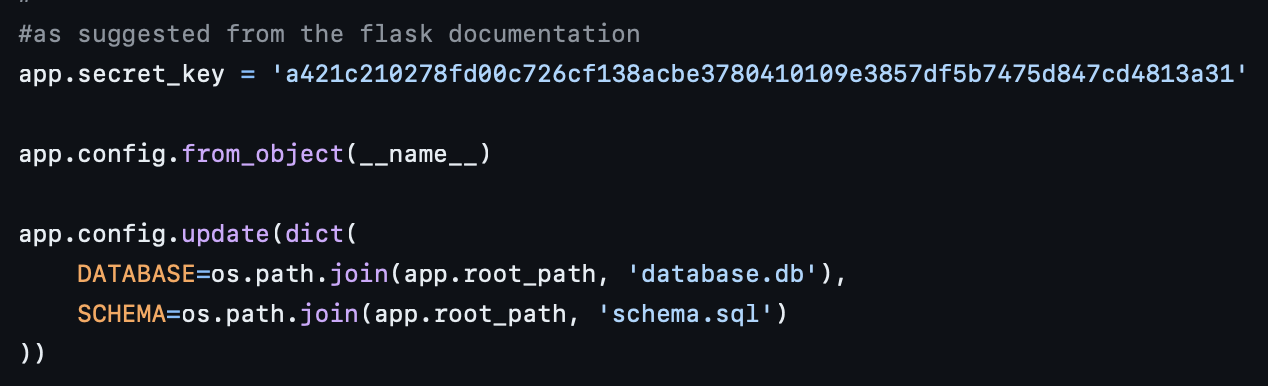
\includegraphics[width=0.9\textwidth]{images/setup_database1.png}
\end{figure}

Questa porzione di codice serve ad impostare quelle che sono le variabili di configurazione per l’inizializzazione e utilizzo del database.

\subsubsection{Connessione con il database}
\begin{figure}[H]
    \centering
    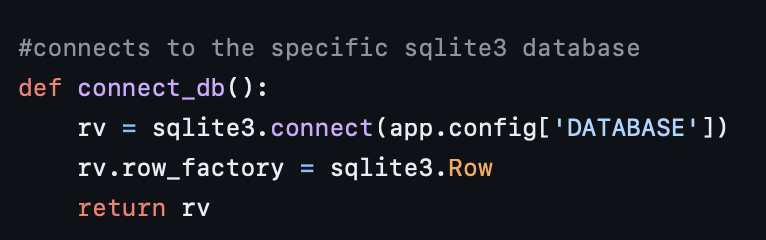
\includegraphics[width=0.9\textwidth]{images/connessione_db.png}
\end{figure}

Questa funzione serve per stabilire una connessione con uno specifico database sqlite3, rv è l’oggetto di connessione al database, che potrà poi essere usato per interagire con lo stesso.

\subsubsection{Aprire una nuova connessione con il database}
\begin{figure}[H]
    \centering
    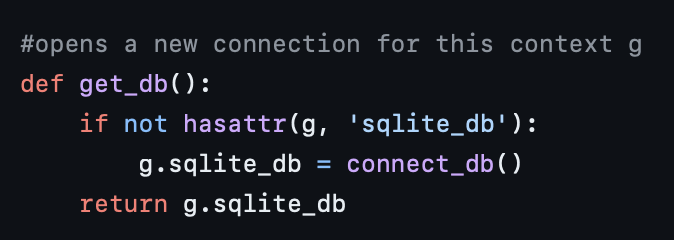
\includegraphics[width=0.9\textwidth]{images/apertura_connessione_db.png}
\end{figure}

Funzione che ci permette, nel caso non fosse già presente, di instaurare una nuova connessione e memorizzarne il contenuto nell’oggetto g, permettendoci così di utilizzarla in diverse parti dell’applicazione.

\subsubsection{Chiusura della connessione}
\begin{figure}[H]
    \centering
    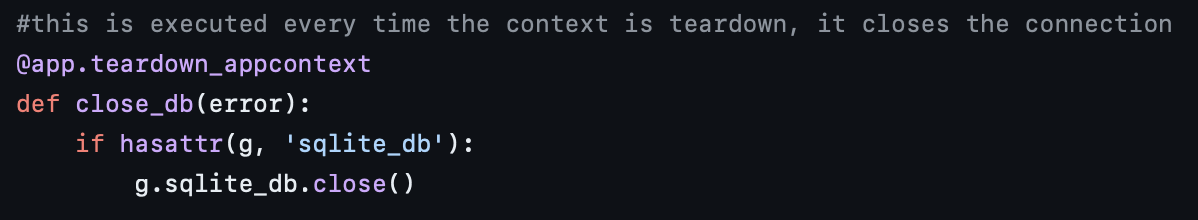
\includegraphics[width=0.9\textwidth]{images/chiusura_connessione_db.png}
\end{figure}

Questa funzione invece serve per concludere la connessione con il database allorché l’applicazione Flask termini di utilizzarlo, in modo da evitare problemi di risorse non rilasciate.

\subsubsection{Inizializzazione del database}
\begin{figure}[H]
    \centering
    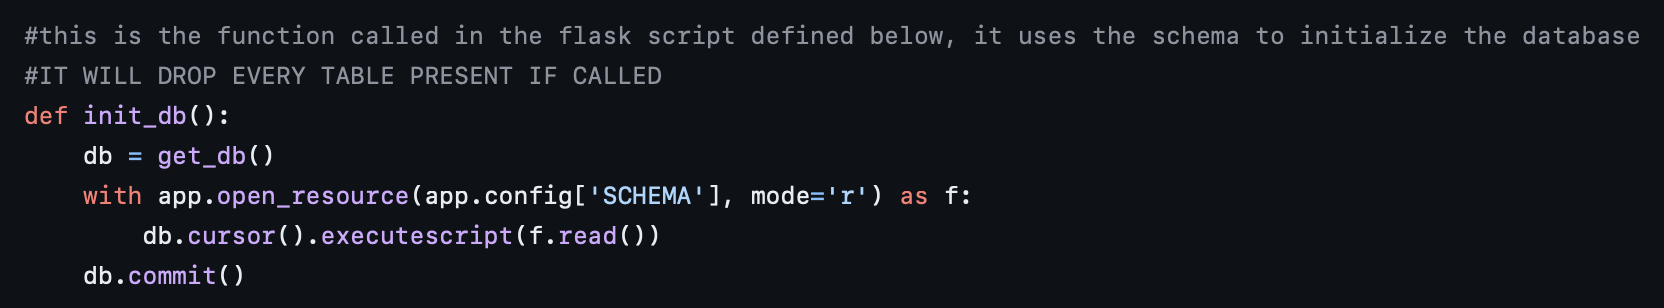
\includegraphics[width=0.9\textwidth]{images/inzializzazione_db.png}
\end{figure}

Questa funzione serve per inizializzare il database all’interno dell’applicazione Flask: prima si invoca la funzione get\textunderscore db in modo da ottenere la connessione con il database, poi andiamo ad aprire il file dello schema, in modalità lettura.
Dopo aver ottenuto un oggetto cursos, andremo ad utilizzare tale oggetto per eseguire lo script che abbiamo letto nel file schema.sql; utilizziamo db.commit per confermare le modifiche appena fatte.



\subsubsection{Inizializzazione da linea di comando}
\begin{figure}[H]
    \centering
    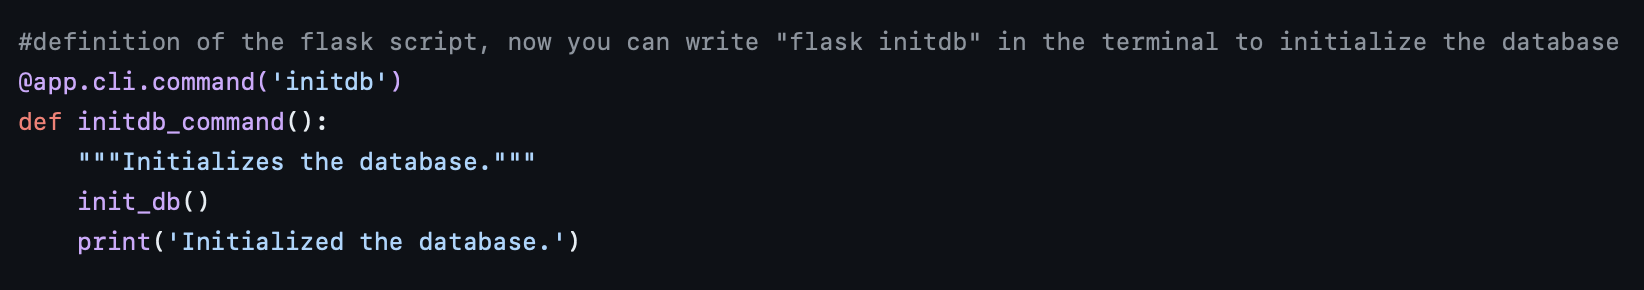
\includegraphics[width=0.9\textwidth]{images/inizializzazione_linea_comando.png}
\end{figure}

Quest’ultima porzione di codice, per quanto riguarda la sezione dedicata al database, ci permette di inizializzare il database tramite linea di comando “flask initdb”. 
Una volta dato questo comando il nostro database sarà inizializzato e pronto per essere utilizzato.

Da tenere in considerazione che tutte le volte che questo comando viene lanciato il database sarà azzerato, perdendo tutti i dati al proprio interno.


\subsection{API}
Ora entriamo nella sezione dedicata alle API, funzioni che ci permettono di comunicare con il nostro client e nelle quali andremo ad utilizzare effettivamente il database che abbiamo creato nella porzione precedente di codice.

\subsubsection{Invio della classifica}
\begin{figure}[H]
    \centering
    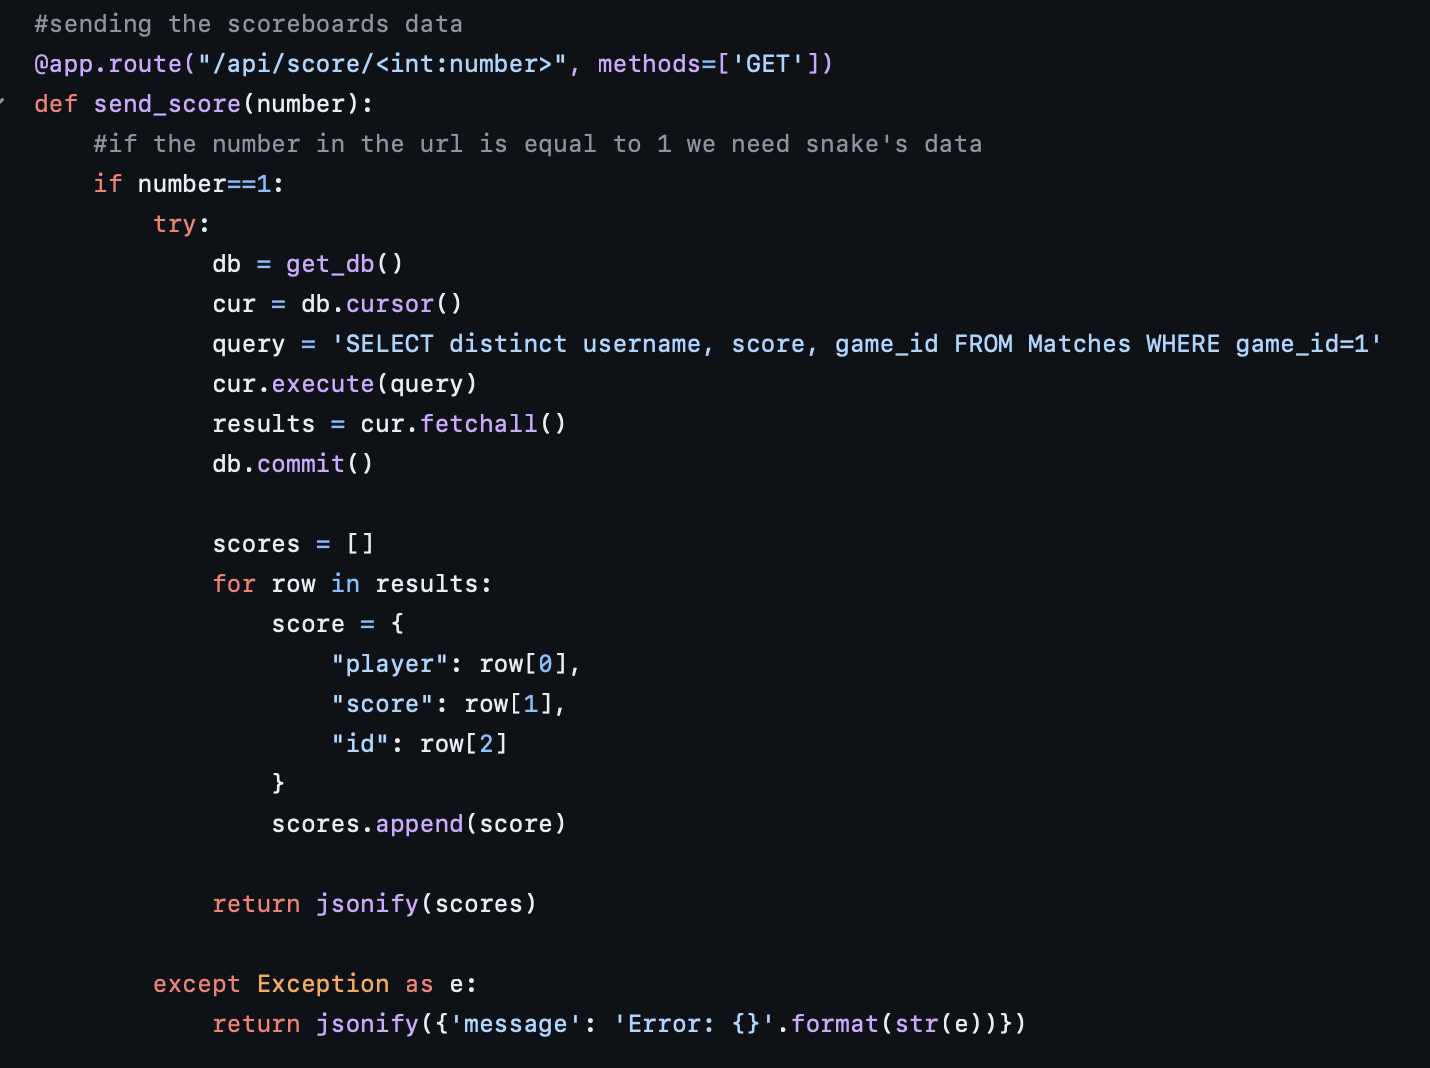
\includegraphics[width=0.9\textwidth]{images/invio_classifica1.png}
\end{figure}

\begin{figure}[H]
    \centering
    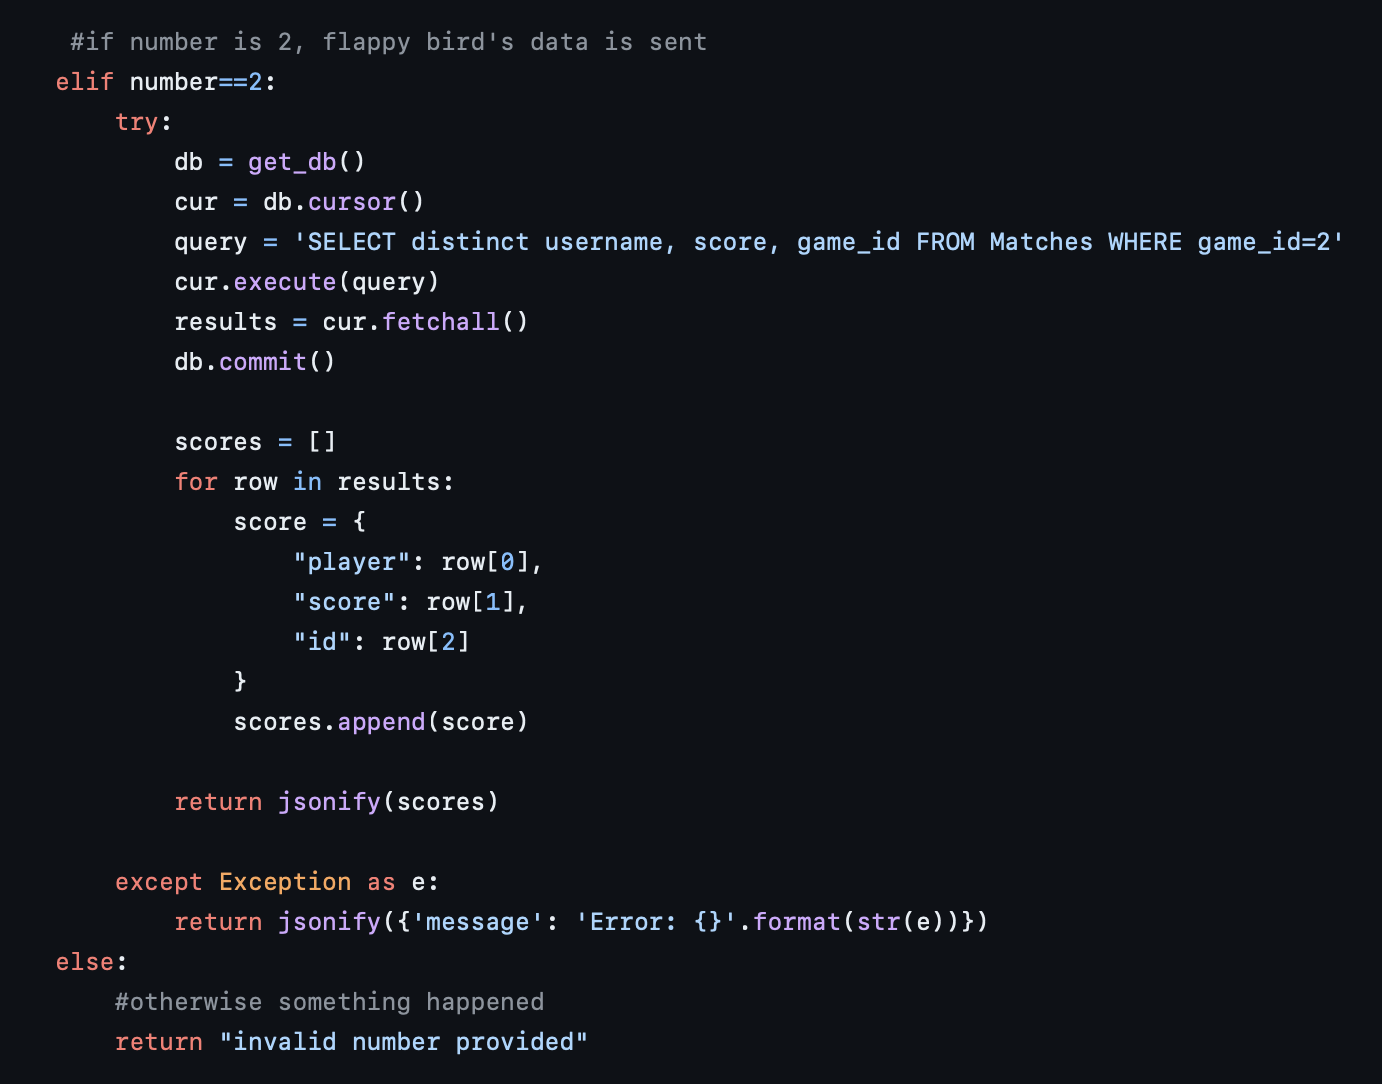
\includegraphics[width=0.9\textwidth]{images/invio_classifica2.png}
\end{figure}
Questa funzione di tipo GET, che quindi invia dati dal server al client, serve per inviare i punteggio, id del gioco, e nome utente, legati tra loro, tenuti nel database, al client in modo da poter mostrare le classifiche divise per gioco.

La richiesta del client avviene ad un url specifico che termina con un valore numero intero, tale valore numerico assume un valore differente per specificare di quale gioco si vuole ricevere i punteggi.

Una volta che abbiamo identificato il gioco, tramite un semplice if statement, dobbiamo andare ad utilizzare le funzioni per instaurare la connessione con il database per poter effettuare la query ed estrarre le informazioni di cui abbiamo bisogno dal database.

Salviamo tutte le tuple ottenute in una variavbile, tramite il metodo fetchll, che che ci consente di tenere tutti i risultati e non solo uno, e poi andiamo a creare una lista di json con i risultati ottenuti; lista che poi inviamo al client tramite apposito metodo.

Il tutto viene fatto in regime di try catch per intercettare un qualunque errore che potrebbe avvenire e notificare di conseguenza il client.

\subsubsection{Salvare il punteggio delle partite}

\begin{figure}[H]
    \centering
    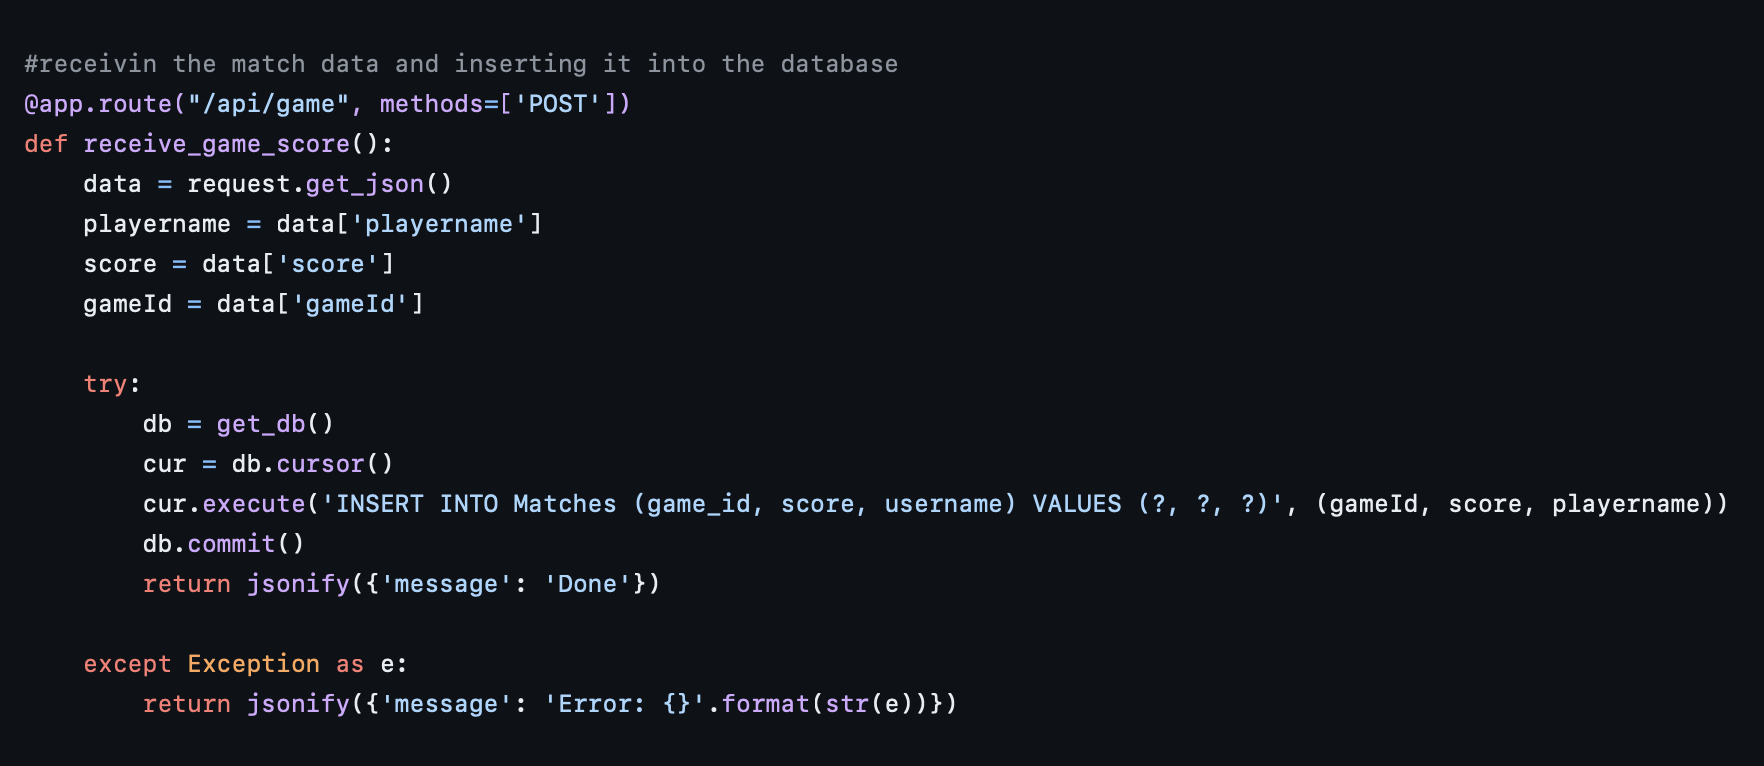
\includegraphics[width=0.9\textwidth]{images/salvare_punteggio_partite.png}
\end{figure}
Questa funzione di tipo POST, che quindi invia dati dal client al server, serve per ricevere e i dati ottenuti da una partita giocata; i dati passati dal client in formato json vengono poi messi nel database tramite la funzione INSERT. 

Queste operazioni vengono tutte eseguite in regime di try catch in modo da intercettare un qualunque errore e notificare il client sia in caso di operazione performata con successo, sia in caso in cui sia avvenuto un errore.

\subsubsection{Controllo accesso di un utente}
\begin{figure}[H]
    \centering
    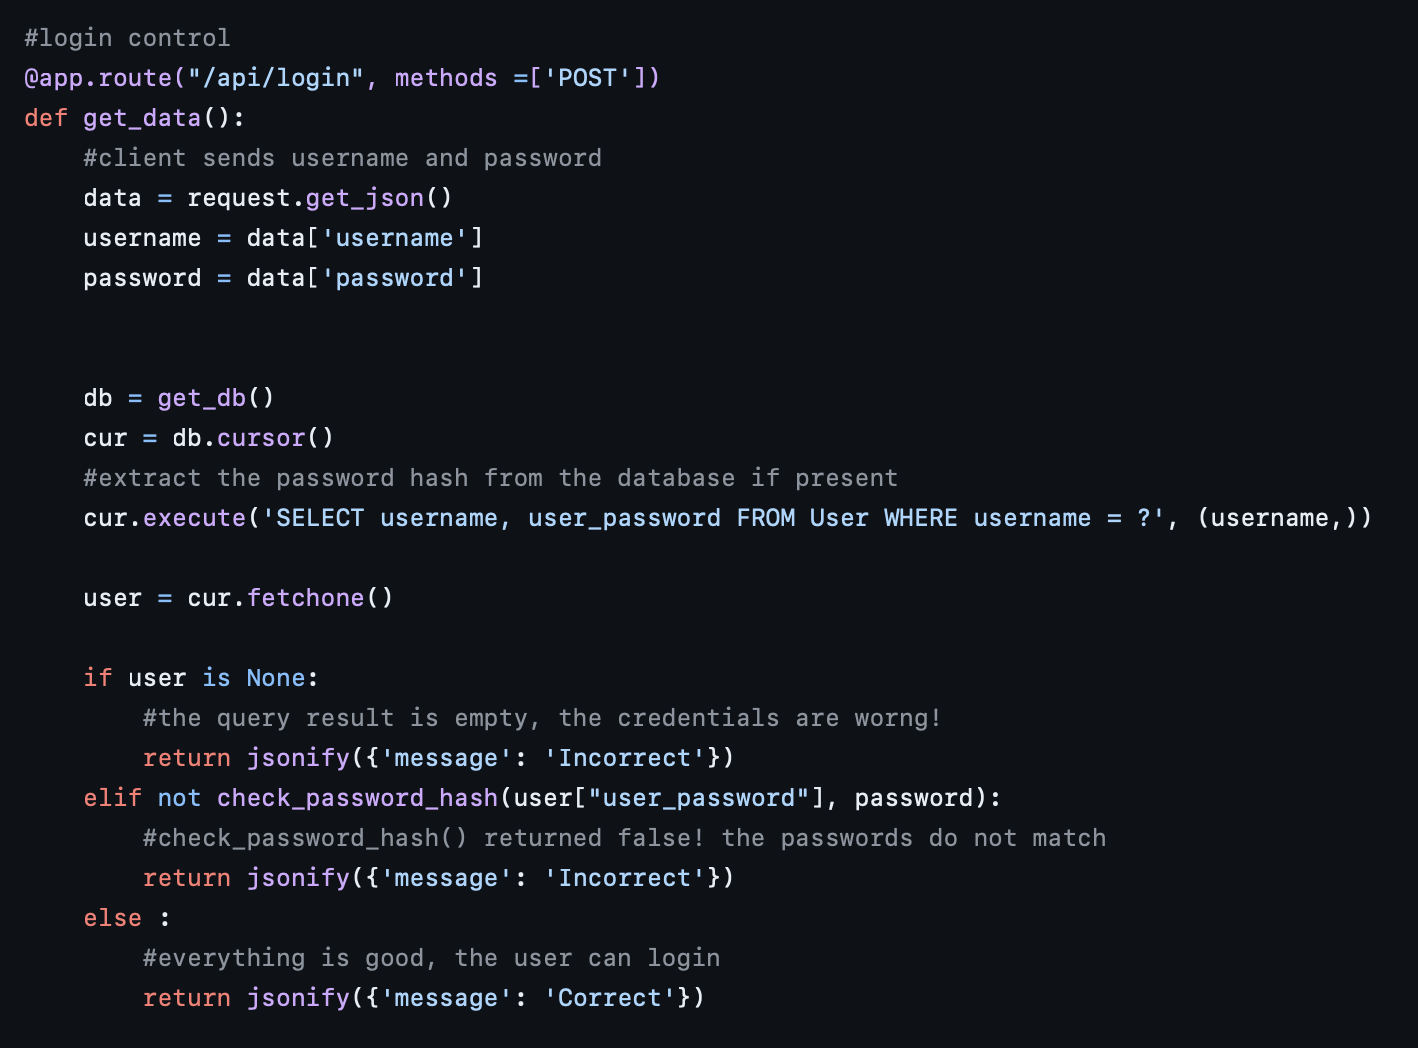
\includegraphics[width=0.9\textwidth]{images/controllo_login.png}
\end{figure}

Questa funzione serve per permettere l’accesso ad utente già registrato.
La funzione riceve dal client il nome utente e la password inseriti: per prima cosa controlla che lo username esista, se esiste allora passiamo a controllare che anche la password, dopo aver usato l’apposita funzione per decriptarla, corrisponda.
Il nome utente è univoco essendo chiave primaria nello schema sql, motivo per cui si usa la fatchone e non la fatchall.

Al termine notifichiamo il client con il risultato che ottenuto dalla verifica.

\subsubsection{Iscrizione nuovo utente}
\begin{figure}[H]
    \centering
    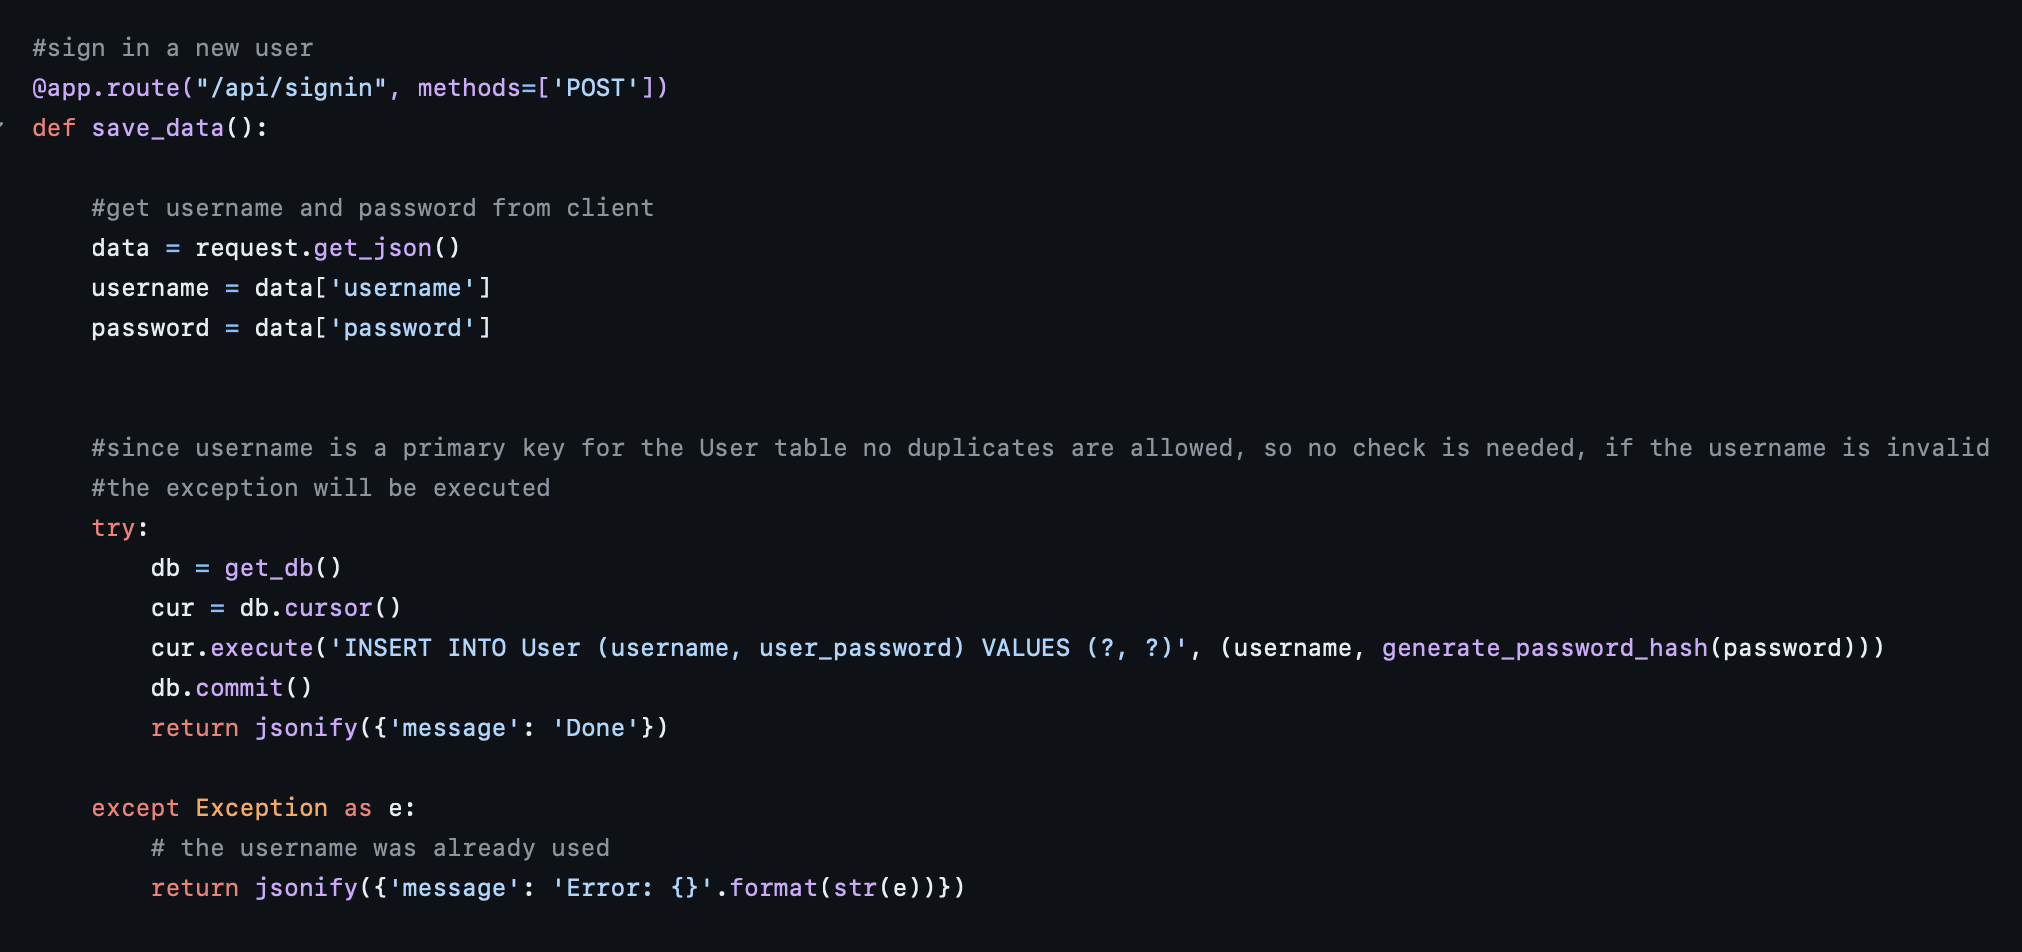
\includegraphics[width=0.9\textwidth]{images/iscrizione_nuovo_utente.png}
\end{figure}

L’ultima funzione che abbiamo è quella per permette ad un nuovo utente di iscriversi: riceviamo ancora una volta il nome utente e la password dal client, sempre in formato json, dopo di che andiamo ad aggiungere questi valori al database.
L’unico errore che possiamo ottenere è che il nome utente sia già presente nel database, essendo chiave primaria non possono essere presenti due nomi utenti uguali, in tal caso andiamo a notificare il client che non siamo riusciti a performare l’operazione richiesta.

\subsubsection{Sezione dedicare all'esecuzione dell'app (facoltativa)}
\begin{figure}[H]
    \centering
    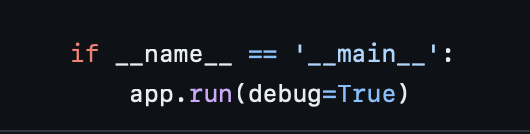
\includegraphics[width=0.9\textwidth]{images/esecuzione_app.png}
\end{figure}

Queste sono le due ultime righe del nostro backend e sono facoltative: ci servono solo per avviare la nostra applicazione e farlo con la modalità debug attiva.



\subsection{Database}
Il nostro database, fatto in sqlite3, ha una struttura relazionale e si basa su tre tabelle sql.
\begin{figure}[H]
    \centering
    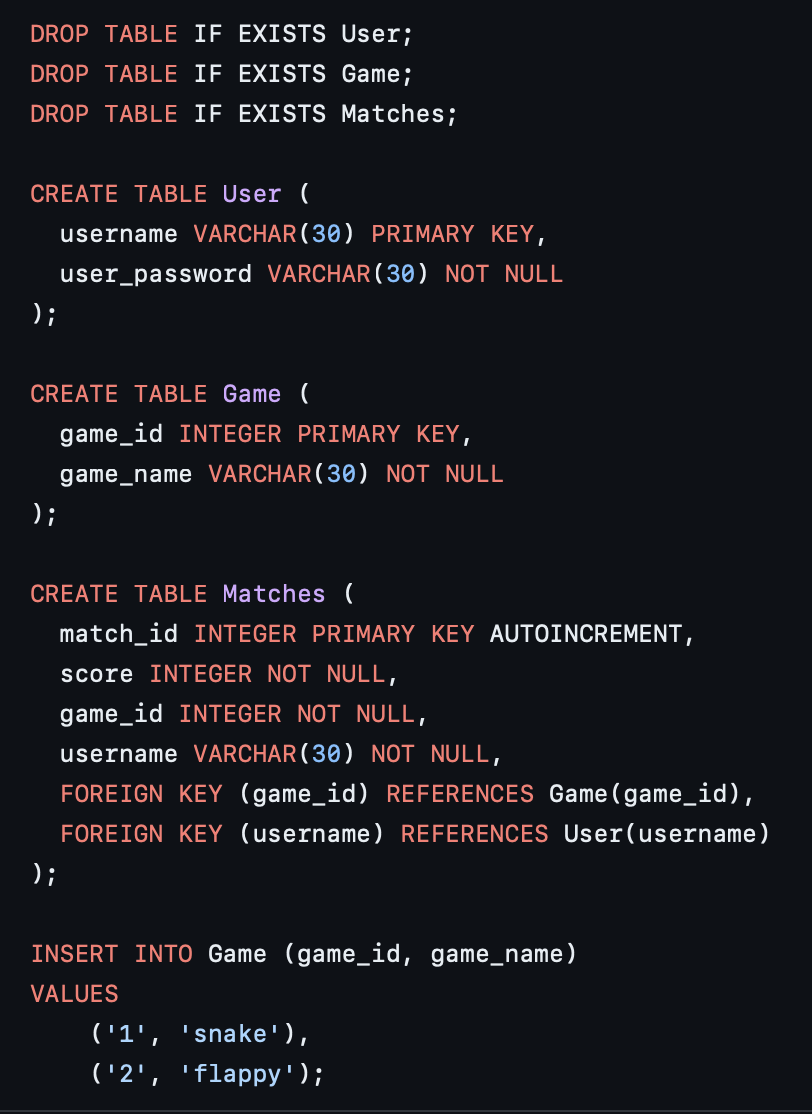
\includegraphics[width=0.9\textwidth]{images/schema_sql.png}
\end{figure}

Andiamo a creare 3 tabelle: User, Game e Matches.

La tabella User è quella che andrà a contenere il nome utente e la password di ogni utente; essendo username chiave primaria questo evita che ci possano essere due utenti con lo stesso nome.

Game invece contiene l’id identificativo associato a ciascun gioco (1 per snake e 2 per flappy) e viene inizializzato direttamente con questi valori al suo interno quando viene creato il database.

Matches è invece la tabella che si occupa di mettere in relazione le altre due: infatti contiene sia lo username che il game\textunderscore id, ma in aggiunta troviamo il match\textunderscore id, valore che identifica in modo univoco ogni partita giocata, e il punteggio ottenuto in tale partita. 
Infine troviamo anche esplicitati i vincoli di integrità referenziale.





\end{document}